\documentclass[11pt,a4paper]{article}
\usepackage[utf8]{inputenc}
\usepackage[T1]{fontenc}
\usepackage{amsmath,amsfonts,amssymb}
\usepackage{graphicx}
\usepackage{booktabs}
\usepackage{array}
\usepackage{multirow}
\usepackage{float}
\usepackage{geometry}
\usepackage{tikz}
\usepackage{pgfplots}
\usepackage{subcaption}
\usepackage{hyperref}
\usepackage{xcolor}
\usepackage{listings}
\usepackage{algorithm}
\usepackage{algorithmic}
\usepackage{tikz-uml}

\geometry{margin=2.5cm}
\pgfplotsset{compat=1.17}

\title{\textbf{HumAIne Evaluation Methodology: Comprehensive Process Diagrams and Scientific Framework}}
\author{Methodology Documentation and Process Visualization}
\date{\today}

\begin{document}

\maketitle

\begin{abstract}
This document provides comprehensive process diagrams and detailed scientific descriptions of the HumAIne chatbot evaluation methodology. The evaluation framework employs systematic virtual persona generation, controlled conversation simulation, and multi-dimensional performance analysis to assess AI-driven personalization capabilities. This paper presents detailed process flows, system architecture diagrams, and algorithmic descriptions that form the foundation of our evaluation approach.
\end{abstract}

\section{Introduction}

The evaluation of personalized conversational AI systems requires a systematic and rigorous methodology to ensure reliable and reproducible results. This document presents the comprehensive process diagrams and scientific framework underlying the HumAIne chatbot evaluation, providing detailed insights into the methodology, system architecture, and evaluation procedures.

\section{Overall System Architecture}

\subsection{High-Level System Overview}

Figure \ref{fig:system_overview} presents the high-level architecture of the HumAIne evaluation framework, illustrating the main components and their interactions.

\begin{figure}[H]
\centering
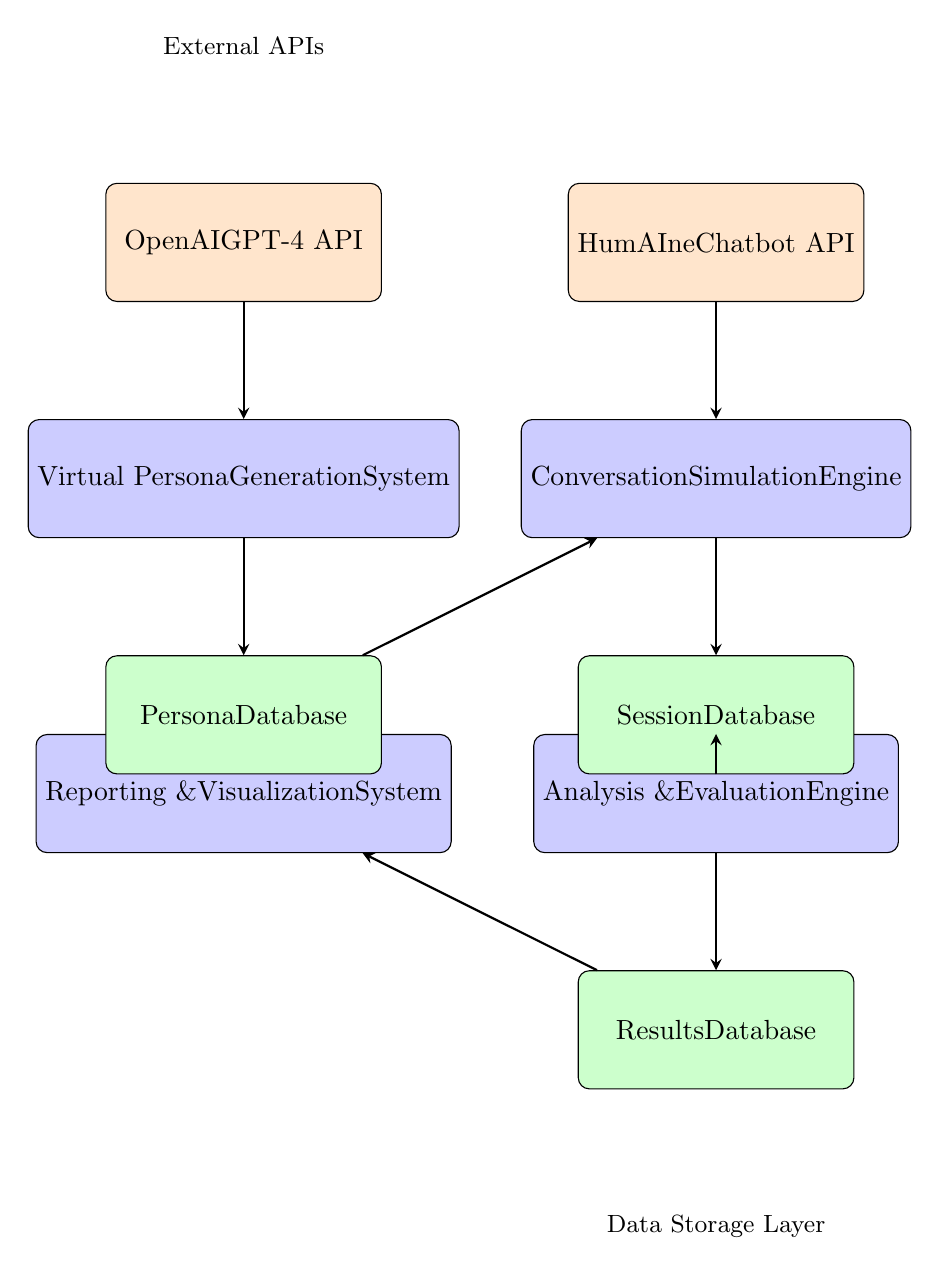
\begin{tikzpicture}[node distance=2cm, auto]
    % Define styles
    \tikzstyle{component} = [rectangle, minimum width=3.5cm, minimum height=1.5cm, text centered, draw=black, fill=blue!20, rounded corners]
    \tikzstyle{data} = [rectangle, minimum width=3.5cm, minimum height=1.5cm, text centered, draw=black, fill=green!20, rounded corners]
    \tikzstyle{api} = [rectangle, minimum width=3.5cm, minimum height=1.5cm, text centered, draw=black, fill=orange!20, rounded corners]
    \tikzstyle{arrow} = [thick,->,>=stealth]
    \tikzstyle{label} = [font=\small]

    % Main components
    \node (persona_gen) [component] {Virtual Persona\\Generation\\System};
    \node (conversation_sim) [component, right of=persona_gen, xshift=4cm] {Conversation\\Simulation\\Engine};
    \node (analysis_engine) [component, below of=conversation_sim, yshift=-2cm] {Analysis \&\\Evaluation\\Engine};
    \node (reporting) [component, left of=analysis_engine, xshift=-4cm] {Reporting \&\\Visualization\\System};

    % Data stores
    \node (persona_db) [data, below of=persona_gen, yshift=-1cm] {Persona\\Database};
    \node (session_db) [data, below of=conversation_sim, yshift=-1cm] {Session\\Database};
    \node (results_db) [data, below of=analysis_engine, yshift=-1cm] {Results\\Database};

    % External APIs
    \node (openai) [api, above of=persona_gen, yshift=1cm] {OpenAI\\GPT-4 API};
    \node (humaine) [api, above of=conversation_sim, yshift=1cm] {HumAIne\\Chatbot API};

    % Arrows
    \draw [arrow] (openai) -- (persona_gen);
    \draw [arrow] (persona_gen) -- (persona_db);
    \draw [arrow] (persona_db) -- (conversation_sim);
    \draw [arrow] (humaine) -- (conversation_sim);
    \draw [arrow] (conversation_sim) -- (session_db);
    \draw [arrow] (session_db) -- (analysis_engine);
    \draw [arrow] (analysis_engine) -- (results_db);
    \draw [arrow] (results_db) -- (reporting);

    % Labels
    \node [label, above of=openai, yshift=0.5cm] {External APIs};
    \node [label, below of=results_db, yshift=-0.5cm] {Data Storage Layer};
\end{tikzpicture}
\caption{High-Level System Architecture of the HumAIne Evaluation Framework}
\label{fig:system_overview}
\end{figure}

\subsection{Detailed Component Architecture}

Figure \ref{fig:detailed_architecture} provides a more detailed view of the system components and their internal structure.

\begin{figure}[H]
\centering
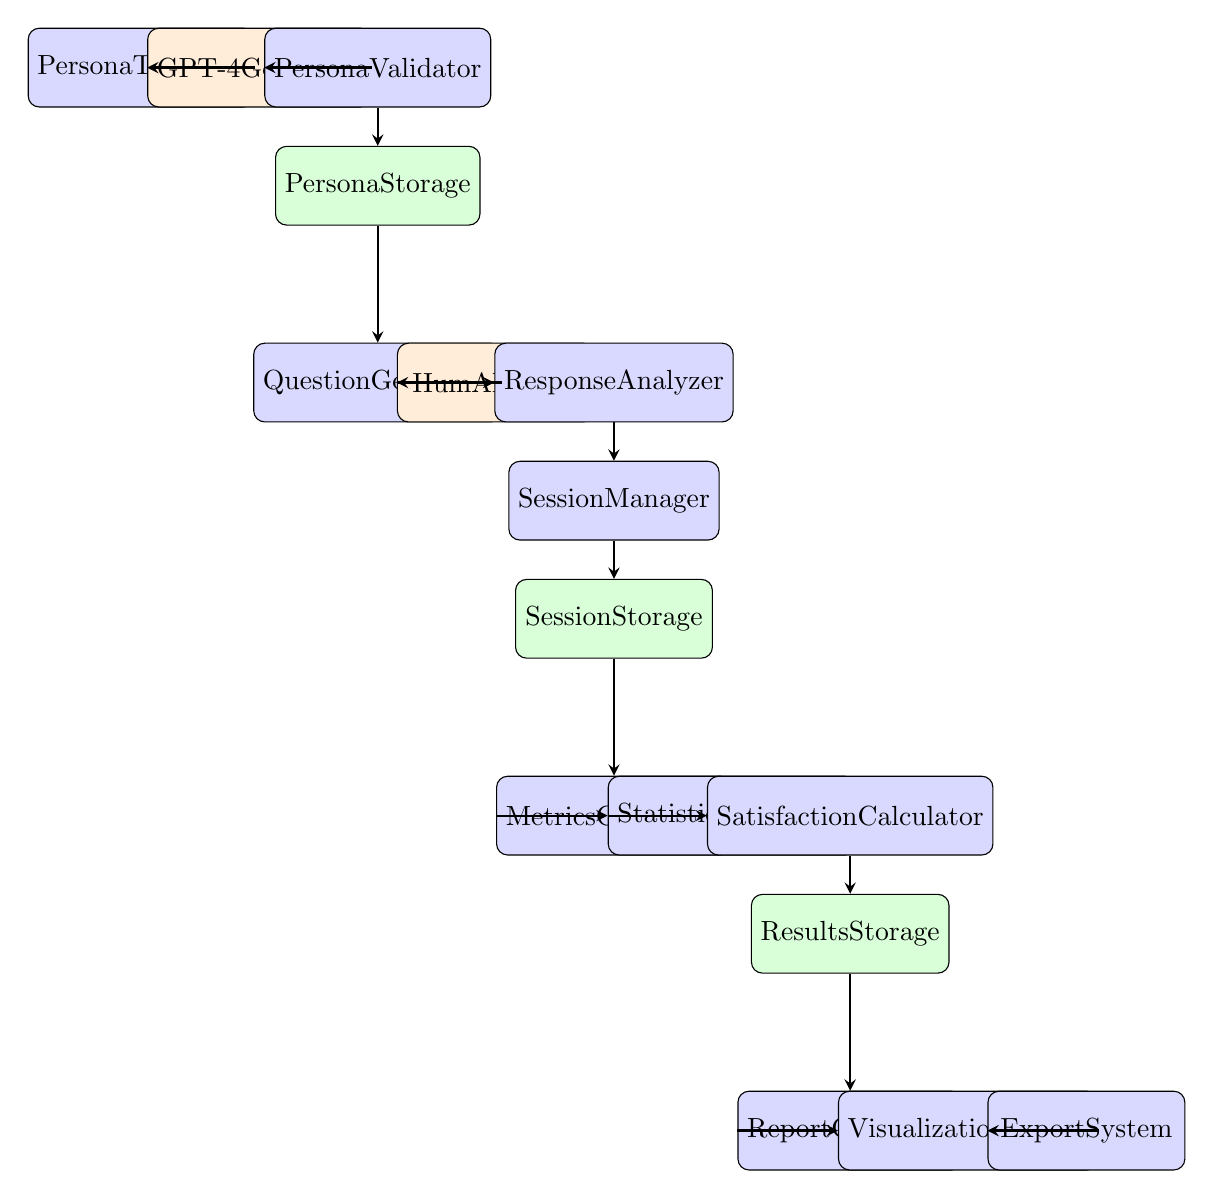
\begin{tikzpicture}[node distance=1.5cm, auto]
    % Define styles
    \tikzstyle{module} = [rectangle, minimum width=2.5cm, minimum height=1cm, text centered, draw=black, fill=blue!15, rounded corners]
    \tikzstyle{storage} = [rectangle, minimum width=2.5cm, minimum height=1cm, text centered, draw=black, fill=green!15, rounded corners]
    \tikzstyle{external} = [rectangle, minimum width=2.5cm, minimum height=1cm, text centered, draw=black, fill=orange!15, rounded corners]
    \tikzstyle{arrow} = [thick,->,>=stealth]

    % Persona Generation Layer
    \node (persona_template) [module] {Persona\\Template};
    \node (gpt4_gen) [external, right of=persona_template] {GPT-4\\Generator};
    \node (persona_validator) [module, right of=gpt4_gen] {Persona\\Validator};
    \node (persona_storage) [storage, below of=persona_validator] {Persona\\Storage};

    % Conversation Simulation Layer
    \node (question_gen) [module, below of=persona_storage, yshift=-1cm] {Question\\Generator};
    \node (humaine_api) [external, right of=question_gen] {HumAIne\\API};
    \node (response_analyzer) [module, right of=humaine_api] {Response\\Analyzer};
    \node (session_manager) [module, below of=response_analyzer] {Session\\Manager};
    \node (session_storage) [storage, below of=session_manager] {Session\\Storage};

    % Analysis Layer
    \node (metrics_calc) [module, below of=session_storage, yshift=-1cm] {Metrics\\Calculator};
    \node (statistical_analyzer) [module, right of=metrics_calc] {Statistical\\Analyzer};
    \node (satisfaction_calc) [module, right of=statistical_analyzer] {Satisfaction\\Calculator};
    \node (results_storage) [storage, below of=satisfaction_calc] {Results\\Storage};

    % Reporting Layer
    \node (report_gen) [module, below of=results_storage, yshift=-1cm] {Report\\Generator};
    \node (viz_engine) [module, right of=report_gen] {Visualization\\Engine};
    \node (export_system) [module, right of=viz_engine] {Export\\System};

    % Arrows
    \draw [arrow] (persona_template) -- (gpt4_gen);
    \draw [arrow] (gpt4_gen) -- (persona_validator);
    \draw [arrow] (persona_validator) -- (persona_storage);
    \draw [arrow] (persona_storage) -- (question_gen);
    \draw [arrow] (question_gen) -- (humaine_api);
    \draw [arrow] (humaine_api) -- (response_analyzer);
    \draw [arrow] (response_analyzer) -- (session_manager);
    \draw [arrow] (session_manager) -- (session_storage);
    \draw [arrow] (session_storage) -- (metrics_calc);
    \draw [arrow] (metrics_calc) -- (statistical_analyzer);
    \draw [arrow] (statistical_analyzer) -- (satisfaction_calc);
    \draw [arrow] (satisfaction_calc) -- (results_storage);
    \draw [arrow] (results_storage) -- (report_gen);
    \draw [arrow] (report_gen) -- (viz_engine);
    \draw [arrow] (viz_engine) -- (export_system);
\end{tikzpicture}
\caption{Detailed Component Architecture of the Evaluation System}
\label{fig:detailed_architecture}
\end{figure}

\section{Evaluation Process Flow}

\subsection{Complete Evaluation Pipeline}

Figure \ref{fig:evaluation_pipeline} illustrates the complete evaluation pipeline from persona generation to final reporting.

\begin{figure}[H]
\centering
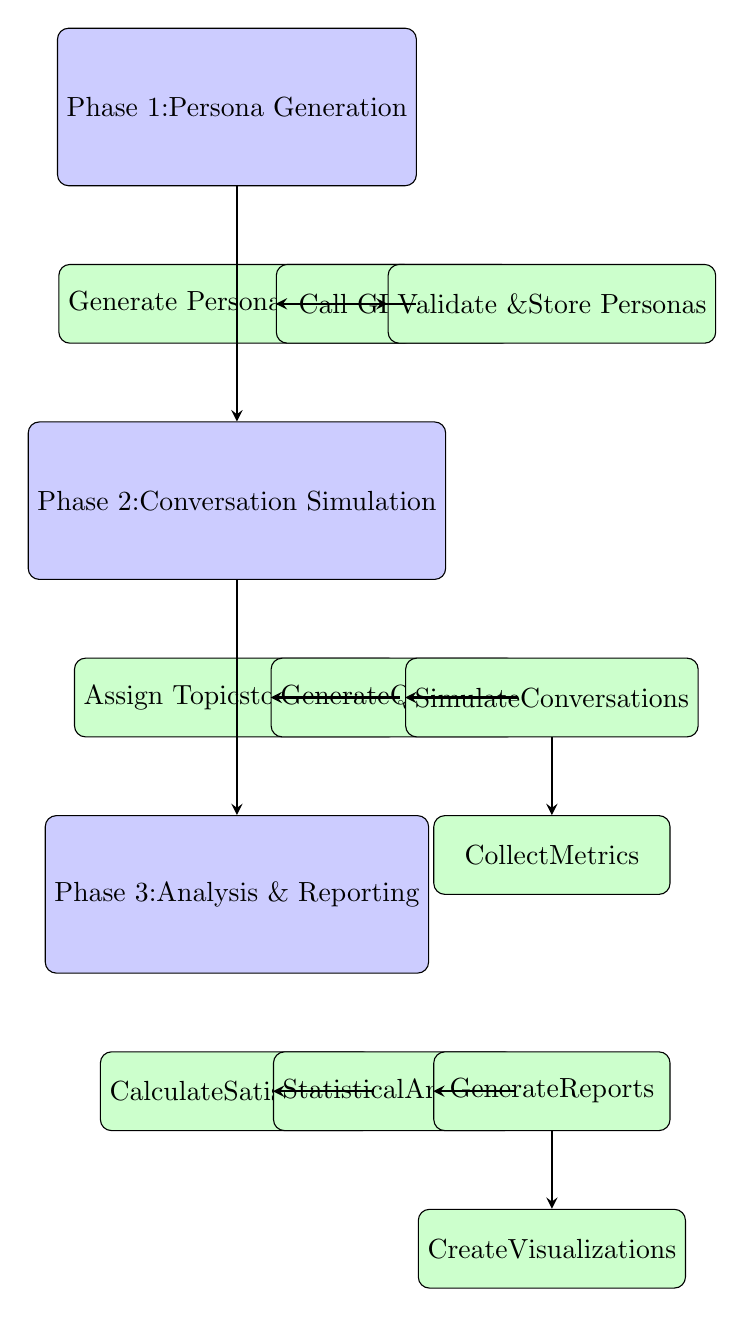
\begin{tikzpicture}[node distance=2cm, auto]
    % Define styles
    \tikzstyle{phase} = [rectangle, minimum width=4cm, minimum height=2cm, text centered, draw=black, fill=blue!20, rounded corners]
    \tikzstyle{process} = [rectangle, minimum width=3cm, minimum height=1cm, text centered, draw=black, fill=green!20, rounded corners]
    \tikzstyle{arrow} = [thick,->,>=stealth]
    \tikzstyle{decision} = [diamond, minimum width=2cm, minimum height=1cm, text centered, draw=black, fill=yellow!20]

    % Phase 1: Persona Generation
    \node (phase1) [phase] {Phase 1:\\Persona Generation};
    \node (p1_1) [process, below of=phase1, yshift=-0.5cm] {Generate Persona\\Templates};
    \node (p1_2) [process, right of=p1_1] {Call GPT-4\\API};
    \node (p1_3) [process, right of=p1_2] {Validate \&\\Store Personas};

    % Phase 2: Conversation Simulation
    \node (phase2) [phase, below of=phase1, yshift=-3cm] {Phase 2:\\Conversation Simulation};
    \node (p2_1) [process, below of=phase2, yshift=-0.5cm] {Assign Topics\\to Personas};
    \node (p2_2) [process, right of=p2_1] {Generate\\Questions};
    \node (p2_3) [process, right of=p2_2] {Simulate\\Conversations};
    \node (p2_4) [process, below of=p2_3] {Collect\\Metrics};

    % Phase 3: Analysis
    \node (phase3) [phase, below of=phase2, yshift=-3cm] {Phase 3:\\Analysis \& Reporting};
    \node (p3_1) [process, below of=phase3, yshift=-0.5cm] {Calculate\\Satisfaction};
    \node (p3_2) [process, right of=p3_1] {Statistical\\Analysis};
    \node (p3_3) [process, right of=p3_2] {Generate\\Reports};
    \node (p3_4) [process, below of=p3_3] {Create\\Visualizations};

    % Arrows between phases
    \draw [arrow] (phase1) -- (phase2);
    \draw [arrow] (phase2) -- (phase3);

    % Arrows within phases
    \draw [arrow] (p1_1) -- (p1_2);
    \draw [arrow] (p1_2) -- (p1_3);
    \draw [arrow] (p2_1) -- (p2_2);
    \draw [arrow] (p2_2) -- (p2_3);
    \draw [arrow] (p2_3) -- (p2_4);
    \draw [arrow] (p3_1) -- (p3_2);
    \draw [arrow] (p3_2) -- (p3_3);
    \draw [arrow] (p3_3) -- (p3_4);
\end{tikzpicture}
\caption{Complete Evaluation Pipeline Process Flow}
\label{fig:evaluation_pipeline}
\end{figure}

\subsection{Persona Generation Process}

Figure \ref{fig:persona_generation_flow} details the persona generation process with decision points and validation steps.

\begin{figure}[H]
\centering
\begin{tikzpicture}[node distance=2cm, auto]
    % Define styles
    \tikzstyle{start} = [ellipse, minimum width=2cm, minimum height=1cm, text centered, draw=black, fill=green!20]
    \tikzstyle{process} = [rectangle, minimum width=3cm, minimum height=1cm, text centered, draw=black, fill=blue!20, rounded corners]
    \tikzstyle{decision} = [diamond, minimum width=2cm, minimum height=1cm, text centered, draw=black, fill=yellow!20]
    \tikzstyle{end} = [ellipse, minimum width=2cm, minimum height=1cm, text centered, draw=black, fill=red!20]
    \tikzstyle{arrow} = [thick,->,>=stealth]

    % Start
    \node (start) [start] {Start Persona\\Generation};

    % Process steps
    \node (init) [process, below of=start] {Initialize Persona\\Template};
    \node (gpt_call) [process, below of=init] {Call GPT-4 API\\with Template};
    \node (validate) [decision, below of=gpt_call] {Validate\\Response?};
    \node (retry) [process, left of=validate, xshift=-3cm] {Retry with\\Modified Prompt};
    \node (store) [process, below of=validate] {Store Persona\\in Database};
    \node (check_count) [decision, below of=store] {50 Personas\\Generated?};
    \node (next_persona) [process, left of=check_count, xshift=-3cm] {Generate Next\\Persona};
    \node (end) [end, below of=check_count] {Persona Generation\\Complete};

    % Arrows
    \draw [arrow] (start) -- (init);
    \draw [arrow] (init) -- (gpt_call);
    \draw [arrow] (gpt_call) -- (validate);
    \draw [arrow] (validate) -- node[left] {No} (retry);
    \draw [arrow] (retry) -- (gpt_call);
    \draw [arrow] (validate) -- node[right] {Yes} (store);
    \draw [arrow] (store) -- (check_count);
    \draw [arrow] (check_count) -- node[left] {No} (next_persona);
    \draw [arrow] (next_persona) -- (init);
    \draw [arrow] (check_count) -- node[right] {Yes} (end);
\end{tikzpicture}
\caption{Persona Generation Process Flow with Validation}
\label{fig:persona_generation_flow}
\end{figure}

\subsection{Conversation Simulation Process}

Figure \ref{fig:conversation_simulation_flow} illustrates the conversation simulation process with detailed interaction steps.

\begin{figure}[H]
\centering
\begin{tikzpicture}[node distance=2cm, auto]
    % Define styles
    \tikzstyle{start} = [ellipse, minimum width=2cm, minimum height=1cm, text centered, draw=black, fill=green!20]
    \tikzstyle{process} = [rectangle, minimum width=3cm, minimum height=1cm, text centered, draw=black, fill=blue!20, rounded corners]
    \tikzstyle{decision} = [diamond, minimum width=2cm, minimum height=1cm, text centered, draw=black, fill=yellow!20]
    \tikzstyle{end} = [ellipse, minimum width=2cm, minimum height=1cm, text centered, draw=black, fill=red!20]
    \tikzstyle{arrow} = [thick,->,>=stealth]

    % Start
    \node (start) [start] {Start Session};

    % Process steps
    \node (load_persona) [process, below of=start] {Load Persona\\Profile};
    \node (assign_topic) [process, below of=load_persona] {Assign Topic\\Domain};
    \node (generate_questions) [process, below of=assign_topic] {Generate Questions\\Based on Persona};
    \node (init_session) [process, below of=generate_questions] {Initialize\\Session};
    \node (question_loop) [decision, below of=init_session] {More Questions\\to Process?};
    \node (send_question) [process, right of=question_loop, xshift=3cm] {Send Question to\\HumAIne API};
    \node (receive_response) [process, below of=send_question] {Receive Chatbot\\Response};
    \node (analyze_response) [process, below of=receive_response] {Analyze Response\\Quality};
    \node (generate_reaction) [process, below of=analyze_response] {Generate Persona\\Reaction};
    \node (store_interaction) [process, below of=generate_reaction] {Store Interaction\\Data};
    \node (calculate_satisfaction) [process, below of=question_loop, yshift=-2cm] {Calculate Session\\Satisfaction};
    \node (store_session) [process, below of=calculate_satisfaction] {Store Session\\Results};
    \node (check_sessions) [decision, below of=store_session] {All Sessions\\Complete?};
    \node (next_session) [process, left of=check_sessions, xshift=-3cm] {Start Next\\Session};
    \node (end) [end, below of=check_sessions] {All Sessions\\Complete};

    % Arrows
    \draw [arrow] (start) -- (load_persona);
    \draw [arrow] (load_persona) -- (assign_topic);
    \draw [arrow] (assign_topic) -- (generate_questions);
    \draw [arrow] (generate_questions) -- (init_session);
    \draw [arrow] (init_session) -- (question_loop);
    \draw [arrow] (question_loop) -- node[above] {Yes} (send_question);
    \draw [arrow] (send_question) -- (receive_response);
    \draw [arrow] (receive_response) -- (analyze_response);
    \draw [arrow] (analyze_response) -- (generate_reaction);
    \draw [arrow] (generate_reaction) -- (store_interaction);
    \draw [arrow] (store_interaction) -- (question_loop);
    \draw [arrow] (question_loop) -- node[right] {No} (calculate_satisfaction);
    \draw [arrow] (calculate_satisfaction) -- (store_session);
    \draw [arrow] (store_session) -- (check_sessions);
    \draw [arrow] (check_sessions) -- node[above] {No} (next_session);
    \draw [arrow] (next_session) -- (start);
    \draw [arrow] (check_sessions) -- node[right] {Yes} (end);
\end{tikzpicture}
\caption{Conversation Simulation Process Flow}
\label{fig:conversation_simulation_flow}
\end{figure}

\section{Satisfaction Scoring Algorithm}

\subsection{Multi-Dimensional Scoring Framework}

Figure \ref{fig:scoring_framework} illustrates the multi-dimensional satisfaction scoring framework.

\begin{figure}[H]
\centering
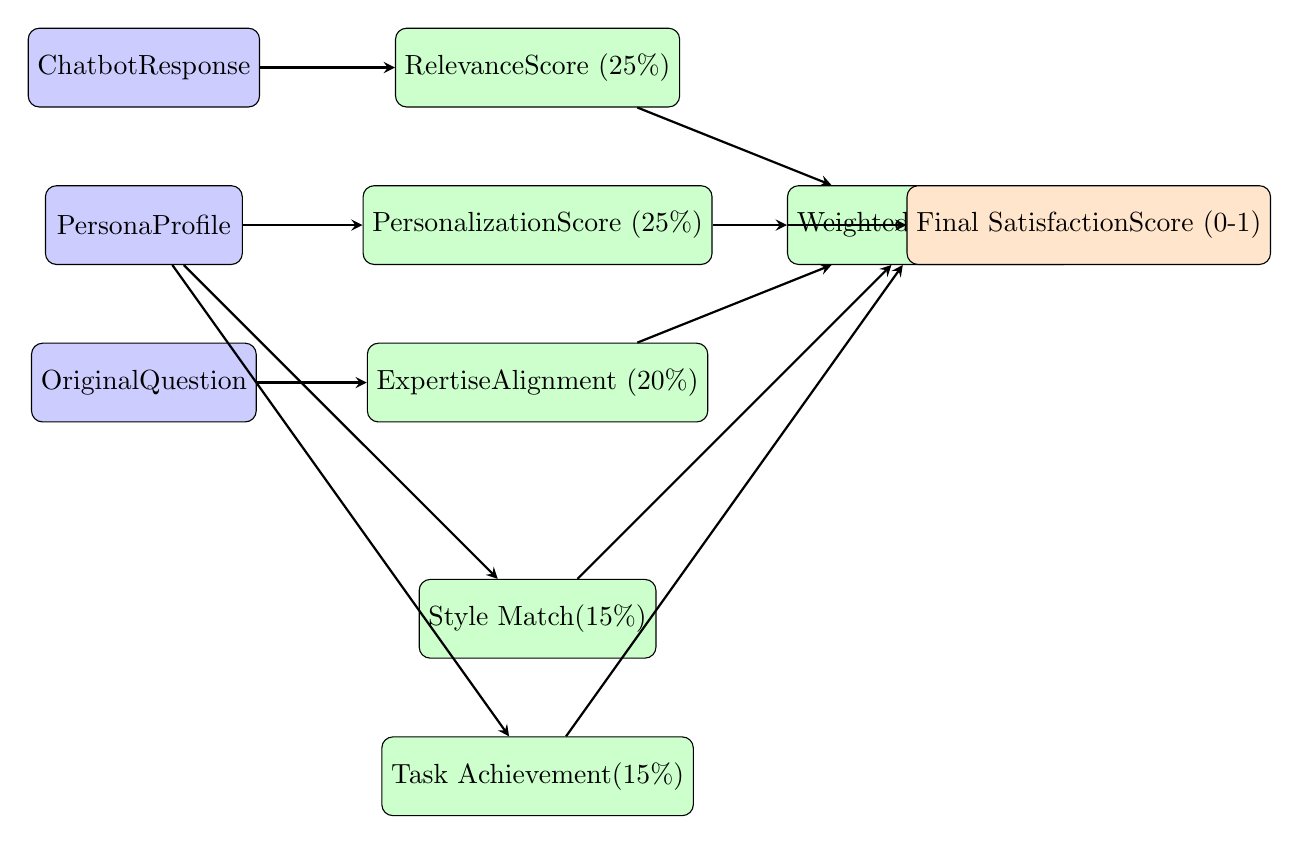
\begin{tikzpicture}[node distance=2cm, auto]
    % Define styles
    \tikzstyle{input} = [rectangle, minimum width=2.5cm, minimum height=1cm, text centered, draw=black, fill=blue!20, rounded corners]
    \tikzstyle{process} = [rectangle, minimum width=2.5cm, minimum height=1cm, text centered, draw=black, fill=green!20, rounded corners]
    \tikzstyle{output} = [rectangle, minimum width=2.5cm, minimum height=1cm, text centered, draw=black, fill=orange!20, rounded corners]
    \tikzstyle{arrow} = [thick,->,>=stealth]

    % Input components
    \node (chatbot_response) [input] {Chatbot\\Response};
    \node (persona_profile) [input, below of=chatbot_response] {Persona\\Profile};
    \node (question) [input, below of=persona_profile] {Original\\Question};

    % Scoring components
    \node (relevance) [process, right of=chatbot_response, xshift=3cm] {Relevance\\Score (25\%)};
    \node (personalization) [process, right of=persona_profile, xshift=3cm] {Personalization\\Score (25\%)};
    \node (expertise) [process, right of=question, xshift=3cm] {Expertise\\Alignment (20\%)};
    \node (style) [process, below of=expertise, yshift=-1cm] {Style Match\\(15\%)};
    \node (task) [process, below of=style] {Task Achievement\\(15\%)};

    % Weighted combination
    \node (weighted_sum) [process, right of=personalization, xshift=3cm] {Weighted\\Combination};
    \node (final_score) [output, right of=weighted_sum] {Final Satisfaction\\Score (0-1)};

    % Arrows
    \draw [arrow] (chatbot_response) -- (relevance);
    \draw [arrow] (persona_profile) -- (personalization);
    \draw [arrow] (question) -- (expertise);
    \draw [arrow] (persona_profile) -- (style);
    \draw [arrow] (persona_profile) -- (task);
    \draw [arrow] (relevance) -- (weighted_sum);
    \draw [arrow] (personalization) -- (weighted_sum);
    \draw [arrow] (expertise) -- (weighted_sum);
    \draw [arrow] (style) -- (weighted_sum);
    \draw [arrow] (task) -- (weighted_sum);
    \draw [arrow] (weighted_sum) -- (final_score);
\end{tikzpicture}
\caption{Multi-Dimensional Satisfaction Scoring Framework}
\label{fig:scoring_framework}
\end{figure}

\subsection{Scoring Algorithm Details}

The satisfaction scoring algorithm is formalized in Algorithm \ref{alg:satisfaction_scoring}.

\begin{algorithm}[H]
\caption{Multi-Dimensional Satisfaction Scoring}
\label{alg:satisfaction_scoring}
\begin{algorithmic}[1]
\REQUIRE Chatbot response $R$, Persona profile $P$, Original question $Q$
\ENSURE Satisfaction score $S \in [0,1]$
\STATE Initialize component scores: $R_{score} = 0, P_{score} = 0, E_{score} = 0, St_{score} = 0, T_{score} = 0$
\STATE \textbf{Calculate Relevance Score} $R_{score}$:
\STATE \quad Extract keywords from $Q$ and $R$
\STATE \quad Compute semantic similarity using word embeddings
\STATE \quad $R_{score} = \text{similarity}(Q, R) \in [0,1]$
\STATE \textbf{Calculate Personalization Score} $P_{score}$:
\STATE \quad Check for persona-specific content in $R$
\STATE \quad Match response style to persona preferences
\STATE \quad $P_{score} = \text{personalization\_level}(R, P) \in [0,1]$
\STATE \textbf{Calculate Expertise Alignment} $E_{score}$:
\STATE \quad Extract domain knowledge from $P$
\STATE \quad Assess response depth and accuracy
\STATE \quad $E_{score} = \text{expertise\_match}(R, P) \in [0,1]$
\STATE \textbf{Calculate Style Match} $St_{score}$:
\STATE \quad Analyze communication style in $P$
\STATE \quad Compare with response tone and formality
\STATE \quad $St_{score} = \text{style\_compatibility}(R, P) \in [0,1]$
\STATE \textbf{Calculate Task Achievement} $T_{score}$:
\STATE \quad Extract current task/goal from $P$
\STATE \quad Assess response helpfulness for task completion
\STATE \quad $T_{score} = \text{task\_helpfulness}(R, P) \in [0,1]$
\STATE \textbf{Calculate Final Score}:
\STATE \quad $S = 0.25 \cdot R_{score} + 0.25 \cdot P_{score} + 0.20 \cdot E_{score} + 0.15 \cdot St_{score} + 0.15 \cdot T_{score}$
\RETURN $S$
\end{algorithmic}
\end{algorithm}

\section{Data Flow Architecture}

\subsection{Information Flow Diagram}

Figure \ref{fig:data_flow} illustrates the complete data flow through the evaluation system.

\begin{figure}[H]
\centering
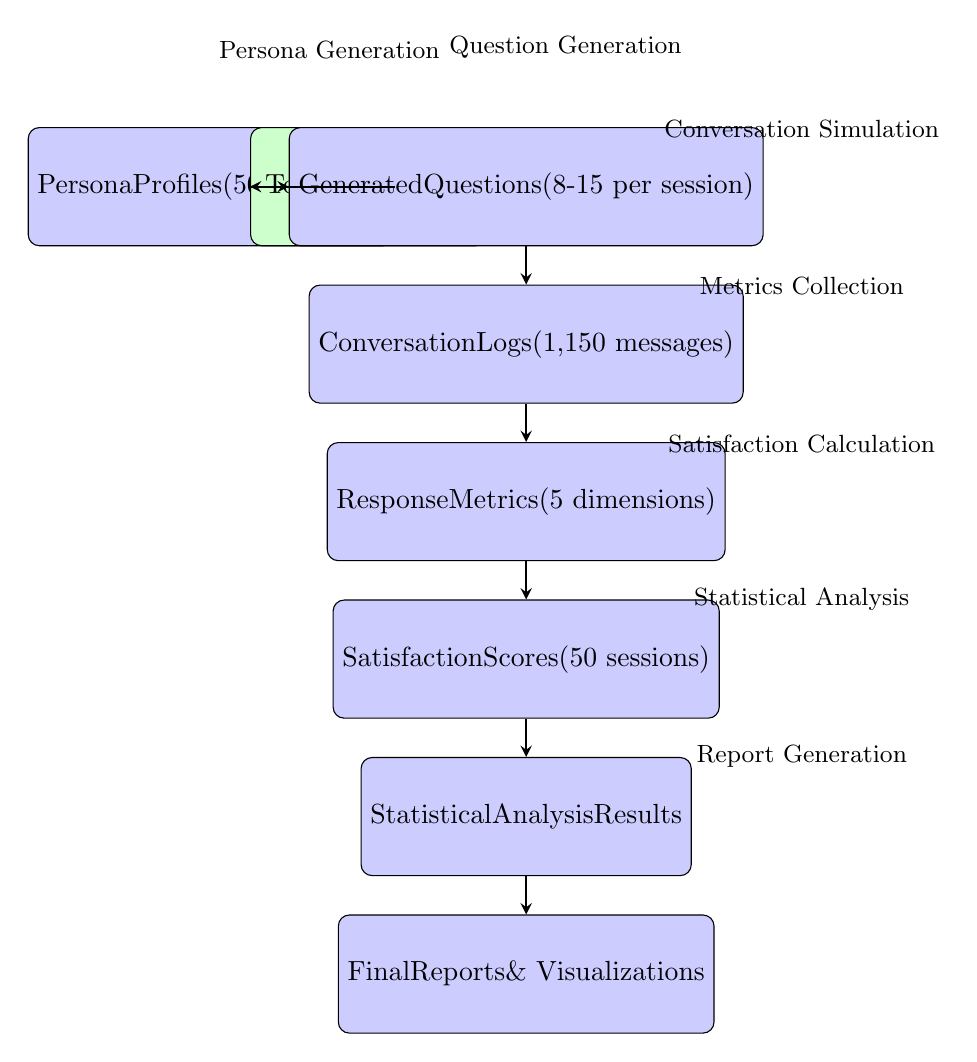
\begin{tikzpicture}[node distance=2cm, auto]
    % Define styles
    \tikzstyle{data} = [rectangle, minimum width=3cm, minimum height=1.5cm, text centered, draw=black, fill=blue!20, rounded corners]
    \tikzstyle{process} = [rectangle, minimum width=3cm, minimum height=1.5cm, text centered, draw=black, fill=green!20, rounded corners]
    \tikzstyle{arrow} = [thick,->,>=stealth]
    \tikzstyle{label} = [font=\small, above]

    % Data flow
    \node (persona_data) [data] {Persona\\Profiles\\(50 personas)};
    \node (topic_assignment) [process, right of=persona_data] {Topic\\Assignment};
    \node (question_data) [data, right of=topic_assignment] {Generated\\Questions\\(8-15 per session)};
    \node (conversation_data) [data, below of=question_data] {Conversation\\Logs\\(1,150 messages)};
    \node (metrics_data) [data, below of=conversation_data] {Response\\Metrics\\(5 dimensions)};
    \node (satisfaction_data) [data, below of=metrics_data] {Satisfaction\\Scores\\(50 sessions)};
    \node (analysis_data) [data, below of=satisfaction_data] {Statistical\\Analysis\\Results};
    \node (reports) [data, below of=analysis_data] {Final\\Reports\\\& Visualizations};

    % Arrows
    \draw [arrow] (persona_data) -- (topic_assignment);
    \draw [arrow] (topic_assignment) -- (question_data);
    \draw [arrow] (question_data) -- (conversation_data);
    \draw [arrow] (conversation_data) -- (metrics_data);
    \draw [arrow] (metrics_data) -- (satisfaction_data);
    \draw [arrow] (satisfaction_data) -- (analysis_data);
    \draw [arrow] (analysis_data) -- (reports);

    % Labels
    \node [label] at (1.5, 1.5) {Persona Generation};
    \node [label] at (4.5, 1.5) {Question Generation};
    \node [label] at (7.5, 0.5) {Conversation Simulation};
    \node [label] at (7.5, -1.5) {Metrics Collection};
    \node [label] at (7.5, -3.5) {Satisfaction Calculation};
    \node [label] at (7.5, -5.5) {Statistical Analysis};
    \node [label] at (7.5, -7.5) {Report Generation};
\end{tikzpicture}
\caption{Complete Data Flow Architecture}
\label{fig:data_flow}
\end{figure}

\subsection{Quality Assurance Framework}

Figure \ref{fig:quality_assurance} illustrates the quality assurance framework integrated throughout the evaluation process.

\begin{figure}[H]
\centering
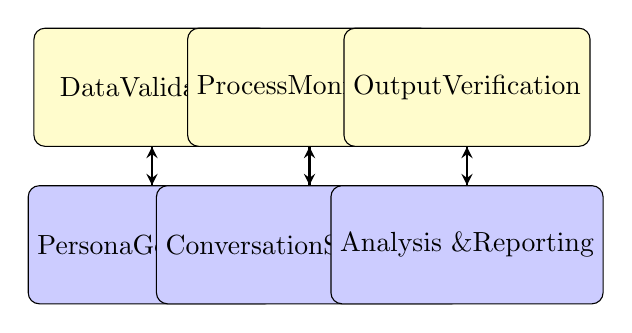
\begin{tikzpicture}[node distance=2cm, auto]
    % Define styles
    \tikzstyle{qa} = [rectangle, minimum width=3cm, minimum height=1.5cm, text centered, draw=black, fill=yellow!20, rounded corners]
    \tikzstyle{process} = [rectangle, minimum width=3cm, minimum height=1.5cm, text centered, draw=black, fill=blue!20, rounded corners]
    \tikzstyle{arrow} = [thick,->,>=stealth]

    % QA components
    \node (data_validation) [qa] {Data\\Validation};
    \node (process_monitoring) [qa, right of=data_validation] {Process\\Monitoring};
    \node (output_verification) [qa, right of=process_monitoring] {Output\\Verification};

    % Processes
    \node (persona_gen) [process, below of=data_validation] {Persona\\Generation};
    \node (conversation_sim) [process, below of=process_monitoring] {Conversation\\Simulation};
    \node (analysis) [process, below of=output_verification] {Analysis \&\\Reporting};

    % Arrows
    \draw [arrow] (data_validation) -- (persona_gen);
    \draw [arrow] (process_monitoring) -- (conversation_sim);
    \draw [arrow] (output_verification) -- (analysis);

    % Feedback arrows
    \draw [arrow, dashed] (persona_gen) -- (data_validation);
    \draw [arrow, dashed] (conversation_sim) -- (process_monitoring);
    \draw [arrow, dashed] (analysis) -- (output_verification);
\end{tikzpicture}
\caption{Quality Assurance Framework}
\label{fig:quality_assurance}
\end{figure}

\section{Scientific Methodology Description}

\subsection{Experimental Design}

The evaluation methodology follows a systematic experimental design with the following key characteristics:

\begin{enumerate}
\item \textbf{Controlled Environment}: All conversations conducted under identical conditions
\item \textbf{Systematic Sampling}: 50 personas with balanced demographic distribution
\item \textbf{Standardized Procedures}: Consistent evaluation protocols across all sessions
\item \textbf{Multi-Dimensional Assessment}: Comprehensive metrics covering multiple aspects of personalization
\item \textbf{Statistical Rigor}: Robust statistical analysis with appropriate significance testing
\end{enumerate}

\subsection{Validity and Reliability}

\subsubsection{Internal Validity}

The evaluation framework ensures internal validity through:
\begin{itemize}
\item Controlled persona generation with standardized templates
\item Consistent conversation simulation procedures
\item Standardized scoring algorithms with defined weights
\item Systematic data collection and validation procedures
\end{itemize}

\subsubsection{External Validity}

External validity is maintained through:
\begin{itemize}
\item Diverse persona demographics representing real user populations
\item Multiple topic domains covering various use cases
\item Realistic conversation scenarios with natural interaction patterns
\item Comprehensive evaluation metrics relevant to real-world applications
\end{itemize}

\subsubsection{Reliability}

Reliability is ensured through:
\begin{itemize}
\item Consistent evaluation procedures across all sessions
\item Standardized scoring algorithms with defined criteria
\item Systematic data validation and quality assurance
\item Reproducible methodology with complete documentation
\end{itemize}

\subsection{Ethical Considerations}

The evaluation framework adheres to ethical principles:
\begin{itemize}
\item Virtual personas eliminate privacy concerns associated with real users
\item Systematic evaluation ensures fair and unbiased assessment
\item Transparent methodology with complete documentation
\item Reproducible results for scientific validation
\end{itemize}

\section{Conclusion}

This comprehensive methodology documentation provides detailed insights into the HumAIne chatbot evaluation framework. The systematic approach, rigorous experimental design, and multi-dimensional assessment ensure reliable and reproducible evaluation of AI-driven personalization capabilities. The detailed process diagrams and algorithmic descriptions establish a foundation for future research and development in conversational AI evaluation.

The methodology's strength lies in its comprehensive coverage of personalization aspects, systematic approach to data collection, and rigorous statistical analysis. This framework provides a benchmark for evaluating conversational AI systems and contributes to the advancement of personalized human-computer interaction research.

\end{document}
